% NUR ZIEL SYSTEM (Das was wir entwickeln) WIE wird mit situationen gearbeitet, was wir machen
\section{Architektur}
Im folgenden Kapitel wird schematisch der gesamte Aufbau der Komponenten erklärt. Es handelt sich hierbei um ein Python Projekt das drei Module besitzt. Die Module sind nach ihren Hauptaufgaben aufgeteilt. Da es sich nicht um eine klassische Applikation handelt, werden die einzelnen Komponenten erläutert.
%
\subsection{Systemaufbau}
Abbildung \ref{fig:system} zeigt den ganzen Systemaufbau dieser Arbeit, wobei der blaue Bereich die Komponenten beinhaltet, die auf unserer Infrastruktur betrieben sind. Das ganze wird auf einem Linux Server gehosted.\\
\begin{figure}[ht]
\centering
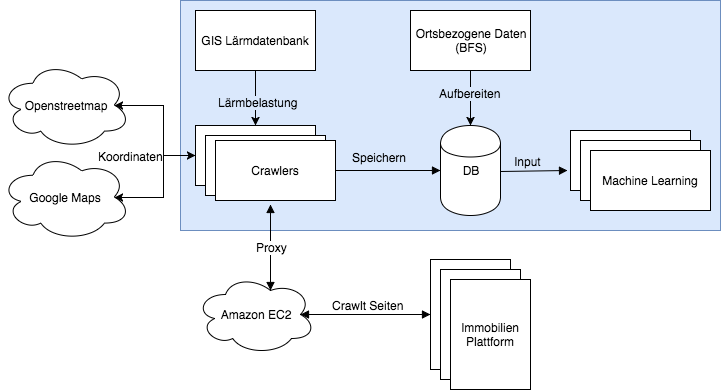
\includegraphics[width=\textwidth]{images/Architektur.png}
\caption[Systemaufbau des Projektes]{Systemaufbau des Projektes}%
\label{fig:system}
\end{figure}
Es gibt diverse Schnittstellen zu externen APIs oder Datenbanken, die wir verwenden um zusätzliche Informationen zu bekommen. Die drei wichtigsten Komponenten sind:
\begin{description}
\item[Crawler:] Sie sammeln die Immobiliendaten auf den verschiedenen Portalen. Die Crawler besitzen diverse Schnittstellen zu anderen Anbieter wie auch Datenbanken. 
\item[Datenbank:] Die Datenbank ist die zentrale Speicherstelle für unsere Inserate. Die Datenbank wurde ganz am Anfang mit ortsbezogenen Daten vom Bundesamt für Statistik befüllt. 
\item[Machine Learning:] Die Daten für das Datenset werden aus der Datenbank geladen und für die verschiedenen Algorithmen bereitgestellt.
\end{description}
In den folgenden Kapiteln wird auf diese drei Komponente genauer eingegangen.
%
\subsection{Aufbau Crawler}
Für diese Arbeit wird Scrapy als Webcrawler verwendet. Scrapy ist ein mächtiges, in Python geschriebenes, Open Source Crawler Framework.\\
Scrapy wurde ausgewählt, da es sich als Python Framework sehr gut in die Entwicklungsumgebung einfügt und es einfach anzuwenden ist \cite{scrapy}.\\
Weiter bietet Scrapy eine Item Pipeline an, um gesammelte Daten weiter zu verarbeiten. Der Vorteil der Pipeline ist, dass es erlaubt unabhängige sowie auch abhängige Schritte der Reihe nach isoliert durchzuführen. Abbildung \ref{fig:scrapy} zeigt den Aufbau der verwendeten Pipeline für das Sammeln von Immobiliendaten.\\[2ex]
\begin{figure}[h!]
\centering

\includegraphics[width=\textwidth]{images/scrapy.png}
\caption[Scrapy Pipeline]{Scrapy Pipeline}%
\label{fig:scrapy}
\end{figure}
\newline
%
\textbf{Crawlen der Webseiten}\\
Für das Crawlen der Kaufobjekte auf einer Immobilienplattform werden fokussierte Crawler verwendet. Da es zahlreiche Immobilienplattformen in der Schweiz gibt, wurden vier der grössten Plattformen ausgesucht, siehe Tabelle(). Die Grösse definiert sich an der Anzahl Inseraten, die auf einer Seite ausgeschrieben sind. Dafür wurde die Rankingliste von Comparis genommen.\\
Um nicht als Crawler aufzufallen wurde mit Scrapoxy auf Amazon mehrere Proxy Instanzen gestartet. Diese wurden im 10-Minuten Takt terminiert und neue gestartet, um immer frische IP-Adressen zu erhalten. Da Amazon keine schweizer Server anbietet, konnten nur Portale angesteuert werden, die ausländische IP-Adressen zulassen. Comparis als grösstes Portal sperrt alle ausländischen IP-Adressen und ist so für uns nicht benutzbar.
